%% LyX 2.0.6 created this file.  For more info, see http://www.lyx.org/.
%% Do not edit unless you really know what you are doing.
\documentclass[british]{book}
\usepackage[T1]{fontenc}
\usepackage[latin9]{inputenc}
\usepackage{geometry}
\geometry{verbose,tmargin=3cm,bmargin=3.7cm,lmargin=3cm,rmargin=2cm,headheight=1cm,headsep=1cm,footskip=0.7cm}
\setcounter{secnumdepth}{3}

\setlength{\parskip}{\medskipamount}
\setlength{\parindent}{0pt}
\usepackage{babel}
\usepackage{array}
\usepackage{verbatim}
\usepackage{refstyle}
\usepackage{booktabs}
\usepackage{textcomp}
\usepackage{url}
\usepackage{multirow}
\usepackage{graphicx}
\usepackage[unicode=true,
 bookmarks=true,bookmarksnumbered=false,bookmarksopen=false,
 breaklinks=false,pdfborder={0 0 1},backref=false,colorlinks=false]
 {hyperref}
 
\hypersetup{pdftitle={Inertial Explorer Manual},
 pdfauthor={Lukasz K Bonenberg},
 pdfsubject={teaching},
 pdfkeywords={Integration, GNSS, IMU, LC}}
\makeatletter
%%%%%%%%%%%%%%%%%%%%%%%%%%%%%% LyX specific LaTeX commands.



%%%%%%%%%%%%%%%%%%%%%%%%%%%%%% User specified LaTeX commands.
%My std preamble for the docs
%\selectlanguage{british}%
\usepackage[british]{babel}
\usepackage{microtype} %better text
\IfFileExists{lmodern.sty}{\usepackage{lmodern}}{} %type 1 vector font
%
\usepackage{lettrine}
\usepackage{listings} %Add list support
\usepackage{colortbl} %colors in TABLES
%\usepackage{tikz,amsmath, amssymb,bm,color}
\usepackage{nicefrac}
\usepackage{lastpage} %get last page

%COLORS
\usepackage{color}
\definecolor{lightgray}{gray}{0.8} %for colortbl
\definecolor{UniBlue}{RGB}{83,121,170}
\definecolor{deepBlue}{HTML}{000066}
\definecolor{blueBgd}{HTML}{99C8FF}
\definecolor{aBlue}{HTML}{1879F7}

%%%%%%%%%%%%%%%%%%%%%%%%%%%%%%%%%%%%%%%%%%%%%%%%%%%%%%%%%%%%%%%%%%
%FOOTNOTES
%nice look after http://www.dedoimedo.com


%%%%%%%%%%%%%%%%%%%%%%%%%%%%%%%%%%%%%%%%%%%%%%%%%%%%%%%%%%%%%%%%%%%
%TABLE SETTINGS
\usepackage{colortbl} %colors in table
\usepackage{rotating} %rotatins within tables
\usepackage{multirow}
\renewcommand{\arraystretch}{1.2} %add padding/spacing
%\usepackage{adjustbox}%rotating and fitting into page
%

\usepackage{booktabs} % To thicken table lines
%define thickness of table lines
\let\mytoprule\toprule
\renewcommand{\toprule}{\mytoprule[0.20em]}
\let\mytoprule\bottomrule
\renewcommand{\bottomrule}{\mytoprule[0.20em]}
\let\mytoprule\midrule
\renewcommand{\midrule}{\mytoprule[0.08em]}

\usepackage{spreadtab} % for simple calculations

%vertically and horizontally centered multicolumn cells with a fixed width. M{width}
%\newcolumntype{M}[1]{>{\centering\hspace{0pt}}m{#1}}
% each spanned cell has the same width. S{width of multicolumn cell}{number of spanned columns}
%\newcolumntype{S}[2]{>{\centering\hspace{0pt}}m{(#1+(2\tabcolsep+\arrayrulewidth)*(1-#2))/#2}}

%%%%%%%%%%%%%%%%%%%%%%%%%%%%%%%%%%%%%%%%%%%%%%%%%%%%%%%%%%%%%%%%%%%
%TikZ
\usepackage{tikz}

\colorlet{red}{red!50}
\colorlet{green}{green!50}
\colorlet{blue}{blue!50}
\definecolor{yellow}{HTML}{FFFF00}
\colorlet{yellow}{yellow!50}
\definecolor{fiolet}{HTML}{7030A0}
\colorlet{fiolet}{fiolet!50}
\colorlet{bgd_main}{black!50}
\colorlet{bgd}{bgd_main!75}
\colorlet{bgd2}{bgd_main!50}
\colorlet{bgd3}{bgd_main!25}
\colorlet{bgd4}{bgd_main!15}

\usetikzlibrary{shapes,arrows,calc,positioning}

%%%%%%%%%%%%%%%%%%%%%%%%%%%%%%%%%%%%%%%%%%%%%%%%%%%%%%%%%%%%%%%%%%%
% Footnotes in Figs
%\rule[raise-height]{width}{thickness}
\newcommand*{\FigFootnote}[1]{
\noindent \begin{flushleft}
\rule[0.2ex]{0.4\columnwidth}{0.5pt}
\par
\footnotesize
#1
\footnotesize
\end{flushleft}
}

%%%%%%%%%%%%%%%%%%%%%%%%%%%%%%%%%%%%%%%%%%%%%%%%%%%%%%%%%%%%%%%%%%%
%MATH, number display
%need to install siunitx, l3kernel,l3packages
\usepackage{siunitx} %this is for units display

\sisetup{per-mode=fraction, tight-spacing = true , fraction-function = \nicefrac, quotient-mode = fraction}% %nicefrac \tfrac
\sisetup{inter-unit-product = \ensuremath { { } \cdot { } } , exponent-product = \cdot }%
\sisetup{input-product=x , output-quotient =  \ensuremath { { } \times{}}} %for 1x2x3
%number grouping(3), std==true %\sisetup{group-digits = decimal} 
\sisetup{group-minimum-digits = 4} %start grouping from 4 digits, in 3 no groups
\sisetup{range-units = single,range-phrase = \,--\,} %2-3C not 2C-3C %, range-phrase = --
\sisetup{separate-uncertainty=true} %2+-1 not 2(1)
\sisetup{prefixes-as-symbols=true } % , scientific-notation = engineering false for 10^-9 ect ect , exp in multiple of 3
\sisetup{range-phrase = \,-\, } % , refo of ranges
%\sisetup{zero-decimal-to-integer, round-mode = places,round-precision = 3}
%\sisetup{add-arc-degree-zero=true , add-arc-minute-zero=true ,add-arc-second-zero=true} %for angle settings

%This is to auto convert ns,ms,us to 10^-xx s
\DeclareSIUnit[scientific-notation = engineering, prefixes-as-symbols=false]{\psec}{\pico\second}
\DeclareSIUnit[scientific-notation = engineering, prefixes-as-symbols=false]{\nsec}{\nano\second} 
\DeclareSIUnit[scientific-notation = engineering, prefixes-as-symbols=false]{\usec}{\micro\second}
\DeclareSIUnit[scientific-notation = engineering, prefixes-as-symbols=false]{\msec}{\milli\second} 

%...AND SOME UNITS
\DeclareSIUnit\dBm{dBm}
\DeclareSIUnit\ppm{ppm} %{\num{1e-6}}%{ppm}
\DeclareSIUnit\yr{yr} %{{361}\day}<-nice nice
\DeclareSIUnit\cy{cycle} %phase cycle
\DeclareSIUnit\epoch{epoch} %GPS/LL epoch
\DeclareSIUnit\inch{"} %inch 
\DeclareSIUnit\wk{week} %week
\DeclareSIUnit\hr{hrs} %hours
\DeclareSIUnit\min{minute} %hours
\DeclareSIUnit\mile{mi}
\DeclareSIUnit\Mcps{Mcps}
\DeclareSIUnit\bit{bit}
\DeclareSIUnit\chip{chip length}
%Other units
\newcommand*{\GBP}[1]{$\SI{#1}[\textsterling]{}$}


%%%%%SHORTHANDS (Standard Sentences)
%\newcommand*{\Myrange}[3]{$\textrm{\SIrange{#1}{#2}{#3}}$}


%how much work per week
\newcommand*{\wkWrk}[1]{$\SI{#1}{\hr\per\wk}$}

%references
\newcommand*{\tabref}[1]{shown in table \ref{#1} on page \pageref{#1}\xspace}
\newcommand*{\vref}[1]{\ref{#1} on page \pageref{#1}\xspace}

 %my math + CROSSREF+nomenclature
%%%%%%%%%%%%%%%%%%%%%%%%%%%%%%%%%%%%%%%%%%%%%%%%%%%%%%%%%%%%%%%%%%%%%%%%
%NOTE boxes
\usepackage{tcolorbox}
\usepackage{lipsum}
%\begin{tcolorbox}[colback=red!25]{NOTES}
\newcommand*{\NOTE}[1]{
	\begin{tcolorbox}[colback=red!25,colframe=red!70!black,title=NOTES]
		{#1}
	\end{tcolorbox}
}

%%%%%%%%%%%%%%%%%%%%%%%%%%%%%%%%%%%%%%%%%%%%%%%%%%%%%%%%%%%%%%%%%%%%%%%%
%SHORTHANDS
%\newcommand*{\Myrange}[3]{$\textrm{\SIrange{#1}{#2}{#3}}$}

%std sentences
\newcommand*{\RefLoc}[1]{Section \vref{#1} provide more information.\xspace}
\newcommand*{\refLoc}[1]{as explained in section \vref{#1}.\xspace}

%HOW 2 reference Wikipedia Common Imaages and others
\newcommand*{\wiki}[1]{ \FigFootnote{Adapted after {#1} / CC BY-SA 3.0}}
\newcommand*{\wikiORG}[1]{ \FigFootnote{Work found at {#1} / CC BY-SA 3.0}}


%defos for GNSS/IMU
\newcommand*{\Q}{symmetric covariance-variance matrix Q\xspace}
\newcommand*{\sday}{Sidereal day is equivalent to $\sdayVal$.\xspace}
\newcommand*{\sdayVal}{$\SI{23.93447}{\hour}$\xspace}
\newcommand*{\IGS}{IGS orbit products\xspace}
\newcommand*{\amb}{the carrier-cycle integer ambiguity\xspace}

%GRID
\newcommand*{\LocalGrid}{Coordinates in the local grid (ENH) using arbitrary conversion and without applying the scale factor.\xspace}
\newcommand*{\OSGB}{Coordinates are in the OSGB grid (ENH), with scale factor applied.\xspace}

 %shortcuts and refs
\AtBeginDocument{
  \def\labelitemii{\(\circ\)}
}
\makeatother

\usepackage{tcolorbox}
\usepackage{lipsum}

%playing with TOC - one page fit
\usepackage{etoolbox}
\makeatletter
\patchcmd{\l@chapter}{1.0em}{0.8em}{}{}
\makeatother


%page xx of xx
\usepackage{lastpage}
\usepackage{fancyhdr}


\begin{document}
\global\long\def\units#1{\textrm{\ensuremath{\mathbf{[\si{#1}]}}}}
%restart numbering for each Part
\makeatletter
\@addtoreset{section}{part}
\makeatother 
\begin{titlepage}
\title{
\includegraphics[width=7cm]{pic/00_logo}\vspace*{5cm}
\\
H24VLP Location Technology\\
\textbf{Project 2}\\
\textbf{Introduction to Inertial Explorer}}
\author{Dr Lukasz Kosma Bonenberg}
\maketitle
\thispagestyle{empty}%no number on this page
\end{titlepage}
\pagebreak{}


%%FRONT MATTER
\frontmatter %to get i,ii
\setcounter{page}{1}

%intro table of content
	
	\setcounter{tocdepth}{2} %how deep are we going to go
	\tableofcontents
	\addtocontents{toc}{~\hfill\textbf{Page}\par} % ?Page? on top of the page numbers in toc/lof/lot

%%%%%%%%%%%%%%%%%%%%%%%%%%%%%%%%% MAIN DOC %%%%%%%%%%%%%%%%%%%%%%%%%%%%%%%%% 
\mainmatter %so we can get proper numbering again


\chapter{Introduction}
\setcounter{page}{1} %start from 1

The goal of this practical is to assess the performance of integrated GNSS and INS for navigation and tracking applications, using a moving platform and to develop a full understanding of the advantages and limitations of integrated GNSS and INS system.\\
To this end you will analyse the performance of three types of IMU sensors (navigation grade, tactical grade and low cost MEMS one) collected during route combining three different environments:
\begin{itemize}
	\item semi-urban;
	\item rural;
	\item dense urban (down town).
\end{itemize}
You will first process GNSS data (as outlined in sections \ref{sec:Processing-GNSS-data}) to create good GNSS trajecotry to be used for processing each IMU separately (section \ref{sec:Processing-Loosely-Coupled}). After obtaining understanding of each system performance you will introduce artificial GNSS denied environment, by introducing gaps (outages) in the GNSS data set (section \ref{sec:Simulating-GNSS-outage}). Duration of those gaps should allow you to properly characterise each of the IMUs and combined with exploratory analysis of all results should allow you to answer the following:\\
\textbf{Characterise the performance of each integrated GNSS and INS system for navigation and tracking applications.}\\
We expect you to both visualise and summarise your work. While a brief description of outputs provided by IE can be found in section \ref{sec:Exporting-final-results}, you are expected to show your own judgement and expertise in selecting output supporting your narrative. It is likely that IE output will be sufficient for that, but you are welcome to summarise some of the results in the tables or plot additional graphs using comparing exported coordinates.

\section{Layout of the practical}
This practical will span two supervised lab classes, giving you knowledge to complete the task. Apart from that, you are expected to work in your own time, and to facilitate this, each group will be provided with two IE dongles for the duration of thee weeks.
\begin{description}
	\item [{Week~1}] Introduction to the practical. By the end you should
	have processed all your GNSS data and started processing IMU data.
	\item [{Week~2}] IMU processing. By the end you should have processed
	all IMU data and start introducing data gaps.
	\item [{Week~3}] Group presentation.
\end{description}

\subsection{Dataset used}

Approximately 90 minutes long dataset was collected using NGI van, equipped with three types of IMU. Trial was run in around Nottingham (see figure \ref{fig:Van-trajectory}). Each dataset should have static period at the beginning and the end, and you will explore both GNSS and IMU data to identify those periods properly. NGB2 was used as a reference station for the duration of the trials. Experiment setup is summarised  in figure \ref{Van-experiment-layout} and table \ref{Lever-Arm-Values}.

All data was converted to \emph{Inertial Explorer} native format. Those files are:
	\begin{description}
	\item [{NGB2.{*}}] GNSS data from NGB2 reference station;
	\item [{POSRS.{*}}] IMU and GNSS data for POSRS receiver (navigation grade);
	\item [{SPAN\_54.{*}}] IMU and GNSS data for SPAN receiver (tactical grade);
	\item [{microstrain.imr}] IMU data for low cost Microstrain receiver;
	\end{description}

\subsection{Handling of data}
During the fist week you will be provided with all relevant data files, which you should copy to local folder on your computer. Please make a backup of all your work before leaving the Photogrammetry Lab. This should include all RAW data files and any \emph{Inertial Explorer} generated files. It is recommended that all project files are placed in the same directory.

\subsection{Supporting Document}

Following document are also provided for your reference:
	\begin{description}
	\item [{POSRS.pdf}] Document outlining POSRS characteristics;
	\item [{SPAN.pdf}] Document outlining SPAN characteristics;
	\item [{Microstrain.pdf}] Document outlining Microstrain characteristics;
	\item [{InertialExplorer850\_Manual.pdf}] Full manual for IE 8.50 (reference
	only).
	\end{description}
	
	
\section{Workflow}
In order to process the data, you will be required to:

\begin{enumerate}
	\item Create a separate project for each IMU (SPAN,	POSRS, MicroStrain);
	\item Process GNSS data, ideally using SPAN receiver, until you satisfied with results;
	\begin{enumerate}
		\item Identify static periods for IMU processing;
		\item Rename final GNSS results as GNSS.cmb.
	\end{enumerate}
	\item Process LC IMU data:
	\begin{enumerate}
		\item Process POSRS, using GNSS.cmb and within static periods ranges, as described in \ref{sub:Processing-POSRS};
		\item Process SPAN, using GNSS.cmb and transferring alignment from POSRS, as described in \ref{sub:Processing-SPAN};
		\item Process Microstrain, using GNSS.cmb and transferring alignment from POSRS, as described in \ref{sub:Processing-Microstrain}).
	\end{enumerate}
	\item Process IMU data only:
	\begin{enumerate}
		\item Process each IMU using transfer alignment as described in section \ref{Processing-IMU-on-its-own};
		\item Draw estimation of required GNSS gaps for each IMU system.
	\end{enumerate}
	\item Introduce GNSS data gaps  as described in section %\ref{Processing-IMU-on-its-own};
	\item Export plots, data ect.
	\item Draw conclusions.
\end{enumerate}



\chapter{Introduction to Inertial Explorer}
Following section explains basics of using IE. If you require additional information please refer to Inertial Explorer Manual provided.



\section{Creating a project}\label{sec:Create-an-new}

You need to create a separate project file for each IMU and put them in the same folder. Please name each project accordingly (SPAN, POSRS, MicroStrain ect).\\
\bigskip

To create a new project open \emph{Inertial Explorer }and go to\textbf{\emph{ File->New Project->Project Wizard}}
\begin{itemize}
	\item Navigate to project folder and create a new project (call it SPAN, POSRS, MicroStrain ect). 
	\item For SPAN project
	\begin{enumerate}
		\item Select required GNSS \& IMU files (SPAN\_54.{*})
		\item antenna height 0m, Measured to APR, use antenna profile as per figure \ref{fig:Van-experiment-layout}
		\item Next
		\item I would like add Base Station Data
		\item Add Station From File
		\item Select NGB2.{*} files as base 
		\item antenna height 0.502m, profile \emph{LEIAR25.R4}
		\item position 52\textdegree{}57'06.95636"N 1\textdegree{}11'02.39879"W 91.2006m
		\item Measured to APR
		\item NEXT, NEXT, Finish, Finish
	\end{enumerate}
	\item For other projects (POSRS, Microstrain)
		\begin{enumerate}
			\item Select required IMU files only ({*}.imr)
			\item antenna height 0m, Measured to APR, use antenna profile as for SPAN
			\item Next
			\item I would like add Base Station Data
			\item Finish, Next, Finish
		\end{enumerate}
\end{itemize}

\section{Processing SPAN GNSS data}\label{sec:Processing-GNSS-data}

As you are only interested in performance of IMU component, you will use the same GNSS data set for each project. To start with check your data overlap using \textbf{\emph{Output->Plot Results}}and selecting\emph{ File Data Coverage }plot. Does rover and base station data overlap? What about IMU data?

\subsection{Precise Clocks/Orbits}
The precise orbits/clocks latency is 12-18 days and the GPS rapid ones its less then a day. If observation are available and you haven't downloaded them in last step, use \textbf{\emph{File->Add precise Files}} 
\begin{itemize}
	\item Set proper time and date, check GLONASS and press Download for combined GPS and GLONASS data (some files will be overwritten);
	\item \emph{Set proper time and date, uncheck GLONASS and press Download for GPS data (clocks are higher resolution then a combined GPS and
	GLONASS ones);}
	\item Press OK to exit window.
	\item In \textbf{\emph{View->Project Overview}} you should be able to see all the files you added.
\end{itemize}

\subsection{Processing GNSS data}

Go to\emph{ }\textbf{\emph{Process->Process GNSS}}
\begin{itemize}
	\item Processing Method: \emph{Differential GNSS;}
	\item Processing Direction: \emph{Both};
	\item Profile GNSS: \emph{Ground Vehicle}, don't change any \emph{Advanced..}
	options;
	\item Add description/User name.
\end{itemize}

To check quality of the position first check overview summary using \textbf{\emph{View->Processing summary}} and then use following plots (\textbf{\emph{output->Plot Results}} or F7): 

\begin{itemize}
	\item Combined Separation
	\item Combined Separation(Fix)
	\item Estimated Position Accuracy
	\item Quality factor
	\item Float/Fixed Ambiguity Status
\end{itemize}

To check baseline data use following plots:

\begin{itemize}
	\item Local Level Vector (pay attention to height component !)
	\item Distance Separation
	\item RMS - Carrier Phase
\end{itemize}

\subsection{Introducing static data in GNSS processing}

For the initialisation of IMU we need to identify static periods at the beginning and end of dataset. We can do using GNSS data only, and also try to improve its accuracy:

\begin{itemize}
\item use \emph{Acceleration Profile} or \emph{Velocity Profile} plots to
identify static periods.
\item create new file Static.txt with each row identifying static period as NAME~START\_TIME~END\_TIME~NOTE (see IE manual page 32 for details). Compare example below: 
	\begin{lstlisting} [language=Matlab,backgroundcolor=\color{lightgray},frame=single,basicstyle=\footnotesize,numbers=left,numbersep=5pt, numberstyle=\tiny\color{mygray}]
		NGI_Start 201200.0 203505.0 Intial_Period_NGB_Yard
		NGI_End 221200.0 223505.0 End_Period_NGB_Yard
	\end{lstlisting}
\item use \textbf{View->GNSS Observations->Remote->Insert Static/Kinematic Markers} and select \textit{Use user generated file to define static periods} to import static data
\item plot \textit{File data coverage} to check if data is properly changed;
\item process GNSS data again
\item Use \emph{Static Session Convergence} plot to assess each period
\item Use any of plots described in previous section to compare results.
\end{itemize}

Once you happy with identified static periods (they should be between 5-10 min long) note beginning and end of whole dataset (that is from first static period to end of last static period identified). Whole processing  generated SPAN.cmb file (combined GPS file). You are going to be using this file later, so please make a copy of it and re-namne it, for example GoodData.cmb. You should not need to re-process GNSS.

\NOTE{
Every plot have menu accessible by right clicking on it. Selecting \emph{Properties }allows to modify plot display\emph{.} Plot range can be modified from same menu using \emph{X-Axis} and \emph{Y-Axis. Apply to All }subcommand match all open plots to the current one.\emph{ Compute statistics for... }provide quantification of plot data. Use \textbf{\emph{Ctr+C}} to copy window content. If you ever close background map, use \textbf{\emph{Output->Show Map window }}.
}


\section{Processing Loosely Coupled GNSS/IMU data\label{sec:Processing-Loosely-Coupled}}

To process  Loosely Coupled GNSS/IMU data use \textbf{\emph{Process->Process LC}}. For every dataset, you should select \textbf{\emph{Advanced->System}} and in \textit{IMU Time Range} input beginning and end of correct dataset (that is from first static period to end of last static period identified in section \ref{sec:Processing-GNSS-data}).

\NOTE{
To verify static periods always plot \emph{File Data Coverage} and \emph{Velocity profile}. Before proceeding check orientation of axis and level arms (those are values AFTER the rotation) are as provided in table \ref{tab:Lever-Arm-Values}. 
}

Following subsection explain settings and workflow for each sensor.

\subsection{Processing POSRS\label{sub:Processing-POSRS}}

In \textbf{\emph{Process->Process LC}} choose:
\begin{description}
	\item [{update~data}] \emph{External Trajectory; }Use \emph{Browser External} to select {*}.cmb file.
	\item [{POSRS~Profile}] \emph{SPAN Airborne (uIRS)}
	\item [{Lever~Arm~Offset}] use POSRS lever arms from table \ref{tab:Lever-Arm-Values} and select \textbf{\emph{Z to ARP}}
	\item [{Body~to~IMU~Rotation:}] \emph{180,0,90 }
	\end{description}
	
\subsubsection{POSRS Workflow\label{sub:POSRS-Workflow}}

\begin{enumerate}
	\item Run all automatic. There should be small separation between pitch and roll (70 arc-sec), aligned with large jumps in heading at the beginning and the end (up to 700 arc-sec). This tend to indicate weak starting (and finishing) angle estimate. Everything else should be smooth (within 70 arc-sec).
	\item Plot \emph{Acceleration Profile} and \emph{Velocity Profile} to check if static periods are matching ones from GNSS only processing. Make sure that dataset start and finish on static period changing \textit{IMU Time Range} in \textbf{\emph{Advanced...}} if necessary.
	\item Knowing static periods go to \textbf{\emph{Advanced...}}and in \textbf{\emph{Method for Initial Alignment}} select \emph{Static Coarse+Fine align} for both reverse and forward. Use Coarse: 60-100s, Fine 100-200s. If you have longer static dataset extend fine alignment period. Results should be within 10 arc-sec and there should be no separation between pitch and roll. There will be large jumps in heading at the beginning and end (up to 100 arc-sec) 
	\item Transfer alignment that is use reverse value for forward solution and vice versa.
	\begin{itemize}
		\item In \textbf{\emph{Advanced...}} for the \textbf{\emph{Method for Initial Alignment}} select \emph{Transfer Alignment (enter known attitude) }and press\emph{ Enter Attitude }button. You will do the same for forward and reverse solution.
		\item Click \emph{Get From Trajectory }and select \emph{reverse} POSRS data ({*}.rim) for forward and \emph{forward} POSRS data ({*}.fim) for reverse. Estimated StdDev for both should be similar. Increase it tenfold (x10) to loosen EKF. 
		\item Click OK
		\item Click \emph{Enter Position and Velocity}, click \emph{ Get from Trajectory} and select the same files (they should be already selected). Click \emph{Extract}.
		\item I suggest increase estimated StdDev tenfold (x10) to loosen EKF. 
		\item Click OK three times to get back to \emph{Process Loosely Coupled} screen.
		\item Process data
	\end{itemize}
	\item Results should be within 10 arc-sec for heading and 2 arc-sec for rest. There should be no separation between pitch and roll. Heading separation should be largest in the middle and no jumps at the beginning/end. 
\end{enumerate}

\subsubsection{Checking results}

To check quality of solution:
\begin{itemize}
	\item To check lever arm in \textbf{\emph{Process->Process LC}} go to \textbf{\emph{Advanced...->States }}and check\emph{ Solve for lever arms. }After reprocessing the data plot\emph{ IMU/IMU-GPS Level Arm} and compare results with values given. Make sure to reprocess data without \emph{Solve for lever arms }for final results and remaining plots.
	\item Plot \emph{Attitude Separation} to check IMU initialisation.
	\item Heading (orientation of axis) can be checked by \emph{IMU Heading COG difference} and \emph{Attitude(Azimuth/Heading)} plots.
	\item To check final position, and quality of LC results plot \emph{Combined Separation, Combined Separation (fix)} and\emph{ IMU/GPS position misclosure}. 
\end{itemize}

\subsection{Processing SPAN}\label{sub:Processing-SPAN}

In \textbf{\emph{Process->Process LC}} select:
\begin{description}
	\item [{update~data:}] \emph{External Trajectory }(select same {*}.cmb
	file as for POSRS processing)
	\item [{SPAN}] Profile: \emph{SPAN Ground (LCI) }
	\item [{Lever~Arm~~Offset}] use SPAN lever arms from table \ref{tab:Lever-Arm-Values}
	\item [{Body2IMU}] Rotation: \emph{0,0,90}
\end{description}

\subsubsection{SPAN Workflow\label{sub:SPAN-Workflow}}

\begin{enumerate}
\item Run all automatic. This is purely to check if data is ok.
\item After checking for static data run \emph{Static Coarse+Fine align}, suggested settings are Coarse: 120s, Fine 480s. If you have longer static dataset extend fine alignment period. Results should show improvement over previous one
\item If all is correct transfer alignment from POSRS as described in section \ref{sub:Processing-POSRS}.
\end{enumerate}

\subsubsection{Checking results}

Same as for POSRS.

\subsection{Processing Microstrain}\label{sub:Processing-Microstrain}

In \textbf{\emph{Process->Process LC}} select:
\begin{description}
	\item [{update~data}] External Trajectory; Use Browser External to select {*}.cmb file.
	\item [{Profile:}] \emph{SPAN Ground (ADIS16488) }
		\begin{itemize}
			\item go to \textbf{\emph{Advanced...->States}}
			\item Under \emph{Error Model} uncheck \emph{Lock Selection} and select \textbf{\emph{Automotive (Low Precision)}} error model
		\end{itemize}
	\item [{Lever~Arm~Offset}] use POSRS lever arms from table \ref{Lever-Arm-Values}
	\item [{Body2IMU}] Rotation: \emph{180,0,90 }
\end{description}

Follow section \ref{SPAN-Workflow} to obtain all results. Bear in mind that this sensor is of much lower accuracy the other ones and it might be more logical to focus on the small set of data.

\section{Processing IMU on its own}\label{Processing-IMU-on-its-own}
After defining starting and ending orientation and position for IMU (using \emph{Transfer Alignment}) it is possible to process IMU only data. To do so:
\begin{enumerate}
	\item In \textbf{Process->Process LC} check \textbf{Process IMU Data only }box;
	\item Depending on desired outcome select Both/Forward/Reverse in \textbf{Processing Direction};
	\item Provide proper description;
	\item Click \textbf{Process}.
\end{enumerate}

\section{Simulating GNSS outage\label{sec:Simulating-GNSS-outage}}

As a part of your assignment you will simulate a GNSS outage. To do this you need to remove epochs from GNSS generated trajectory (see section \ref{sec:Processing-GNSS-data} for more details). Each epoch is saved in following record

\begin{lstlisting} [language=Matlab,backgroundcolor=\color{lightgray},frame=single,basicstyle=\footnotesize,numbers=left,numbersep=5pt, numberstyle=\tiny\color{mygray}]
Out {Tim: 121252.00 121252.000000 1777 			  %GPS second HHMMSS.SSS GPS Week
Geo: 52 57 07.03189 -1 11 00.40441 80.5757 0.061 	%vehicle location
Loc: 37.235 2.335 -10.564 0.054 -0.028 -0.002 	
Sta: 2 0.025500 1.31 1.420 0.960 1.040 	
Rms: 0.0282 2.180 0.000 0.023 0.0406 7.880 1.126 	
Var: 3.85994e-003 6.52259e-004 ...	
Ecf: -7.457 37.397 -7.025 	
Acc: -0.010 0.013 0.025 	
Flg: K L 7 6 	
Sep: 0.136 -0.211 0.151 0.069 0.108 0.077 	
Wgt: 2 2 39 61 	
Cov: -4.00800e-004 7.41043e-005 ...
}
\end{lstlisting}

Delete \emph{Out\{...\}} to remove whole epoch. Make sure you don't remove static data used by IMU to initialise. Start with small data gaps and slowly increase their duration. Make sure you copy and rename relevant {*}.cmb file and you work on COPY! I suggest experimenting with different settings of \textbf{Processing Direction} in \textbf{Process->Process LC} to fully understand system accuracy.



\section{Exporting final results\label{sec:Exporting-final-results}}

\subsection{Graphical results}

To save all active plots use\textbf{\emph{ Output->Build HTML Report }}\emph{. }Data will be saved in .\textbackslash{}Html folder. Save and check all the plots listed in this walk-trough. You should have at least two set of plots (testing and final) for each sensor!  To output trajectory to Google Earth use\textbf{\emph{ Output->Export to Google Earth...}}


In case of multiple exports it recommended to change the output parameters. To do so right click on the background map window, go to \textbf{\emph{Export}} tab and set the following:
\begin{description}
	\item [{Optimize~output~for~trajectory~comparison~in~GE}] creates new colour for the each export (it also means that export don\textquoteright{}t follow Quality Numbers any more), files are not overwritten and a new folder is created if the \emph{Run} descriptor has changed.
	\item [{Use~concise~epoch~description~for~lower~memory~usage}] shortens output information allowing for quick display in Google Earth
\end{description}

First and last option of this menu (\emph{Hold epochs and events to ground }and \emph{Output MSL height for better compatibility with GE elevation data, using}) are mutually exclusive and should be used respectively for terrestrial (ground) and aviation data only.

\subsection{Coordinates}


\NOTE{
	To use \textbf{\emph{Export Wizard}} combined solution ({*}.cmb) must exist. It is generated after each LC/TC processing run but it can be also created using \textbf{\emph{Process->Combine Solution}}. Use extreme caution if using this option.
}

To output post-processed coordinates as ASCII go to \textbf{\emph{Output->Export Wizard}} 	
\begin{itemize}
	\item Select output profile. 
	\begin{itemize}
		\item Mostl likely you will create your own profile using Modify or New buttons.
		\item I suggest outputting either in local grid (East, North, Ellipsoidal Heigh) or Absolute ECEF-XYZ.
		\item Once happy click OK and Next
		\NOTE{
			IE does not produce correct OSGB coordinates. For this experiment you can compare in any grid coordinates, including quasi-OSGB, as long as you mention it. For any other assignment, to obtain those export data as ECEF XYZ and convert it to OSGB use Grid InQuest\footnote{\url{http://www.ordnancesurvey.co.uk/docs/gps/grid-inquest-executable.zip}}.
		}
	\end{itemize}
	\item Select \textbf{\emph{Use processing datum}} and click Next
	\item In this window you define your output parameters
	\begin{itemize}
		\item Define time interval for output (you can interpolate up to 200Hz with POSRS/SPAN but I would recommend outputs of few Hz to keep file sizes reasonable)
		\item Define lever arm using table \ref{tab:Lever-Arm-Values} but read following note in this section before proceeding. 
	\end{itemize}
	
	\NOTE{
		If you followed instruction correctly, your GNSS and IMU level arm will be calculated to antenna ARP but output lever arm will be estimated to antenna phase centre. This means that for EXPORT ONLY your level arm has to be calculated using equation $Arm_{exprt}^{Z}=Arm^{Z}-AntProfile_{L1}^{Z}-AntHeight$. Relevant Arm values can be read from table \ref{tab:Lever-Arm-Values} and antenna profile (\textbf{View->Project Overview}).
	}
	
	
	\item Uncheck \emph{View ASCII} and click \emph{Finish}.
\end{itemize}




\subsection{Checking results}
Check IMU solution against GNSS one. Export values at ARP (\textbf{SUBTRACT antenna L1 height offsets}). It should agree to few mm in clean environment.  Check between different IMU solutions. SPAN/POSRS should agree on mm to cm level.



%%%%%%%%%%%%%%%%%%%%%%%%%%%%%%%APPENDIX

\chapter{Appendixes}
\begin{figure}[tbh]
\centering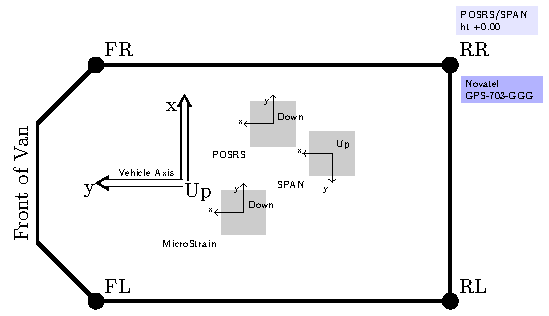
\includegraphics[clip,width=12cm]{pic/VanLayout}%%\resizebox{!}{\textheight}
\caption{Van experiment layout\label{fig:Van-experiment-layout}}
\end{figure}
\begin{figure}[tbh]
\centering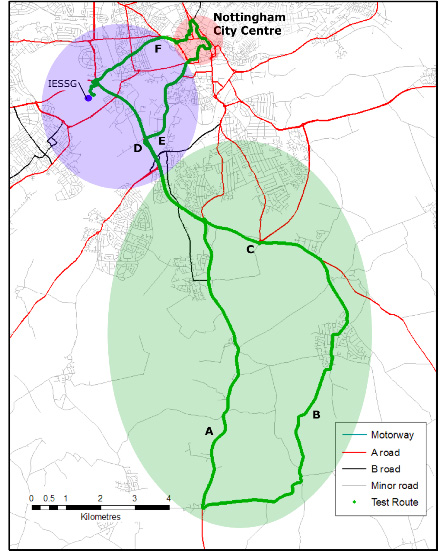
\includegraphics[clip,height=12cm]{pic/TrajectoryLayout}%%\resizebox{!}{\textheight}
\caption{Test route plan\label{fig:Van-trajectory}}
\end{figure}
\begin{table}[h]
\centering{}%
\begin{minipage}[t]{1\columnwidth}%
\begin{center}
\begin{tabular}{>{\centering}m{2.5cm}>{\centering}p{2cm}>{\centering}p{3cm}>{\centering}p{3cm}>{\centering}p{3cm}}
\toprule 
\rowcolor{lightgray}Sensor & \multirow{2}{2cm}{Antenna Location} & \multicolumn{3}{>{\centering}p{9cm}}{Lever Arm%
\footnote{Lever arm is estimated to the ARP. Direction IMU to antenna.%
}}\tabularnewline
\rowcolor{lightgray} &  & X & Y & Z\tabularnewline
\midrule
\multirow{2}{2.5cm}{\textbf{POSRS}} & RR & 0.198 & -0.830 & 0.552\tabularnewline
\cmidrule{2-5} 
 & FL & -1.134 & 2.338 & 0.557\tabularnewline
\midrule
\multirow{2}{2.5cm}{\textbf{SPAN }} & RR & 0.307 & -0.626 & 0.543\tabularnewline
\cmidrule{2-5} 
 & FL & -1.025 & 2.542 & 0.583\tabularnewline
\bottomrule
\end{tabular}\caption{Lever Arms for POSRS and SPAN\label{tab:Lever-Arm-Values}}
\par\end{center}%
\end{minipage}
\end{table}
\begin{table}[h]
\centering{}%
\begin{minipage}[t]{1\columnwidth}%
\begin{center}
\begin{tabular}{>{\centering}p{2cm}>{\centering}p{3cm}>{\centering}p{6cm}>{\centering}p{3cm}}
 \rowcolor{lightgray}\textbf{QN} & \textbf{Color} & \textbf{Description} & \textbf{3D Accuracy (m) }\tabularnewline
\midrule
\textbf{1} & \textcolor{green}{Green}%
\footnote{Suggested accuracy for quality testing\label{fn:Suggested-accuracy-QT}%
} & Fixed integer & $\SIrange[range-phrase=\,-\,]{0.00}{0.15}{}$\tabularnewline
\textbf{2} & \textcolor{cyan}{Cyan} \textsuperscript{\ref{fn:Suggested-accuracy-QT}} & Converged float or noisy fixed integer & $\SIrange[range-phrase=\,-\,]{0.05}{0.40}{}$\tabularnewline
\midrule
\textbf{3} & \textcolor{blue}{Blue} & Converging float & $\SIrange[range-phrase=\,-\,]{0.20}{1.00}{}$\tabularnewline
\textbf{4} & \textcolor{purple}{Purple} & Converging float & $\SIrange[range-phrase=\,-\,]{0.50}{2.00}{}$\tabularnewline
\midrule
\textbf{5} & \textcolor{magenta}{Magenta}%
\footnote{Not recommended for LC\label{fn:Not-recommended-LC}%
} & DGPS & $\SIrange[range-phrase=\,-\,]{1.00}{5.00}{}$\tabularnewline
\textbf{6} & \textcolor{red}{Red}\textsuperscript{\ref{fn:Not-recommended-LC}} & DGPS & $\SIrange[range-phrase=\,-\,]{2.00}{10.00}{}$\tabularnewline
\midrule
 & \textcolor{gray}{Grey} & Not processed & \tabularnewline
 \endrule
\end{tabular}\caption{IE Quality Number description\label{tab:Quality-Number-description}}
\par\end{center}%
\end{minipage}
\end{table}
\begin{comment}
	\begin{table}[h]
	\centering{}%
	\begin{minipage}[t]{1\columnwidth}%
	\begin{center}
	\begin{tabular}{>{\raggedright}m{2.5cm}>{\centering}p{3cm}>{\centering}p{3cm}>{\centering}m{3cm}}
	\rowcolor{lightgray} & \multicolumn{2}{>{\centering}p{6cm}}{\textbf{Duration of GNSS outage {[}s{]}}%
	\footnote{Artificially generated, no valid GNSS information.%
	}} & \multirow{4}{3cm}{\begin{sideways}
	\textbf{Drift value {[}m{]}}%
	\footnote{Value is estimated as double the observed difference (to compensate
	for fwd/rev).%
	}
	\end{sideways}}\tabularnewline
	\cmidrule{2-3} 
	\rowcolor{lightgray} & \textbf{100} & \textbf{300} & \tabularnewline
	\cmidrule{1-3} 
	\multirow{1}{2.5cm}{\textbf{POSRS}} & 0.16 & 1.2 & \tabularnewline
	\cmidrule{1-1} 
	\multirow{1}{2.5cm}{\textbf{SPAN }} & 0.60 & 2.8 & \tabularnewline
	\cmidrule{1-3} 
	\end{tabular}\caption{Approximate positional drift value per GNSS outage}
	\par\end{center}%
	\end{minipage}
	\end{table}
	\begin{table}[h]
	\centering{}%
	\begin{minipage}[t]{1\columnwidth}%
	\begin{center}
	\begin{tabular}{>{\centering}p{2.5cm}c>{\centering}p{1.5cm}>{\centering}p{1cm}>{\centering}p{1cm}>{\centering}p{1cm}>{\centering}p{1cm}>{\centering}m{3cm}}
	 & \multicolumn{6}{c}{\textbf{Duration of GNSS outage {[}s{]}}%
	\footnote{Artificially generated, no valid GNSS information.%
	}} & \multirow{6}{3cm}{\begin{sideways}
	\textbf{Drift value {[}m{]}}
	\end{sideways}}\tabularnewline
	 & \multicolumn{3}{c}{\textbf{One way}} & \multicolumn{3}{c}{\textbf{Combined (Two ways)}} & \tabularnewline
	 & \textbf{56} & \textbf{92} & \textbf{401} & \textbf{56} & \textbf{92} & \textbf{401} & \tabularnewline
	\cmidrule(lr){1-1}\cmidrule(rl){2-4}\cmidrule(rl){5-7}\textbf{POSRS} & 0.30? & N/A & 6.83 & 0.30 & 1.60 & 0.91 & \tabularnewline
	\textbf{SPAN } & 0.80 & 2.90 & 127 & 0.43 & 1.50 & 6.83 & \tabularnewline
	\rowcolor{lightgray}\textbf{Microstrain} &  &  &  & 258 & 255 & 2500 & \tabularnewline
	\cmidrule{1-1} 
	\end{tabular}\caption{IMU positional drift during er GNSS outage, based on 2014 results}
	\par\end{center}%
	\end{minipage}
	\end{table}
\end{comment}
\end{document}
